\documentclass{article}
% \usepackage[spanish]{babel}
% \usepackage{lipsum}
% \usepackage{natbib}
% \usepackage{graphicx}
\usepackage{analysis_orax}

\usepackage{amsmath}
\usepackage{amssymb}


%-------------------------TitlePage------------------------
%\begin{titlepage}
%\end{titlepage}

\title{STA-3001 : COMPUTER-INTENSIVE STATISTICS ASSIGNMENT 3: APPROXIMATION AND OPTIMIZATION}
\author{Gutama Ibrahim}

%------------------Document----------------------------

\begin{document}
\maketitle
%-------------------------Content------------------------

\section*{1 :EM, MCEM, DA}


\begin{description}
	\item[a)]
		The $L(\lambda|y)=L(\lambda|x,z)$\\
	Since we assume all failure times of all individual light bulbs are independent\\
	\begin{align*}
		L(\lambda|y)&=L(\lambda|x)*L(\lambda|z)\\
				&=\{\prod_{i=1}^m f_x(x|\lambda)\}\{\prod_{i=m+1}^n f_z(z|\lambda)\}\\
			&=\{\prod_{i=i=m}^m \lambda^2 x_i e^{-x_i\lambda} \}\{ \prod_{i=m+1}^n \lambda^2 z_i e^{-z_i \lambda}\}
	\end{align*}


The complete log-likelihood
	\begin{align*}
		L(\lambda|y)&=\prod_{i=1}^n x_i \prod_{i=m+1}^n z_i\bigg(\lambda^{2*n} e^{-\lambda(\sum_{i=1}^m x_i +\sum_{i=m+1}^n z_i)} \bigg)
	\end{align*}

	\begin{align*}
		l(\lambda|y)&=\sum_{i=1}^m \ln(x_i)+\sum_{i=m+1}^n \ln(z_i) + 2n \ln \lambda - \lambda \sum_{i=1}^m x_i -\lambda \sum_{i=m+1}^n z_i
	\end{align*}	
			
	\item[b)]
		\begin{align*}
		We have exponen
		E[Z_i|x,\lambda)&=
		\end{align*}
	\item[c)]
	\item[d)]
	\item[e)]
	\item[f)]
	\item[g)]
		
\end{description}

\section*{2:EM}
\begin{description}
	\item[a)]
	\item[b)]
	\item[c)]
	\item[d)]
	\item[e)]
\end{description}



\section*{3:MCI, Reimann,Laplace}


\begin{description}
	\item[]
	
\end{description}


\section*{4:Simulated Annealing}


















































\end{document}


























































\subsection{Subtitle}

    \begin{figure}[htb]
    \centering
      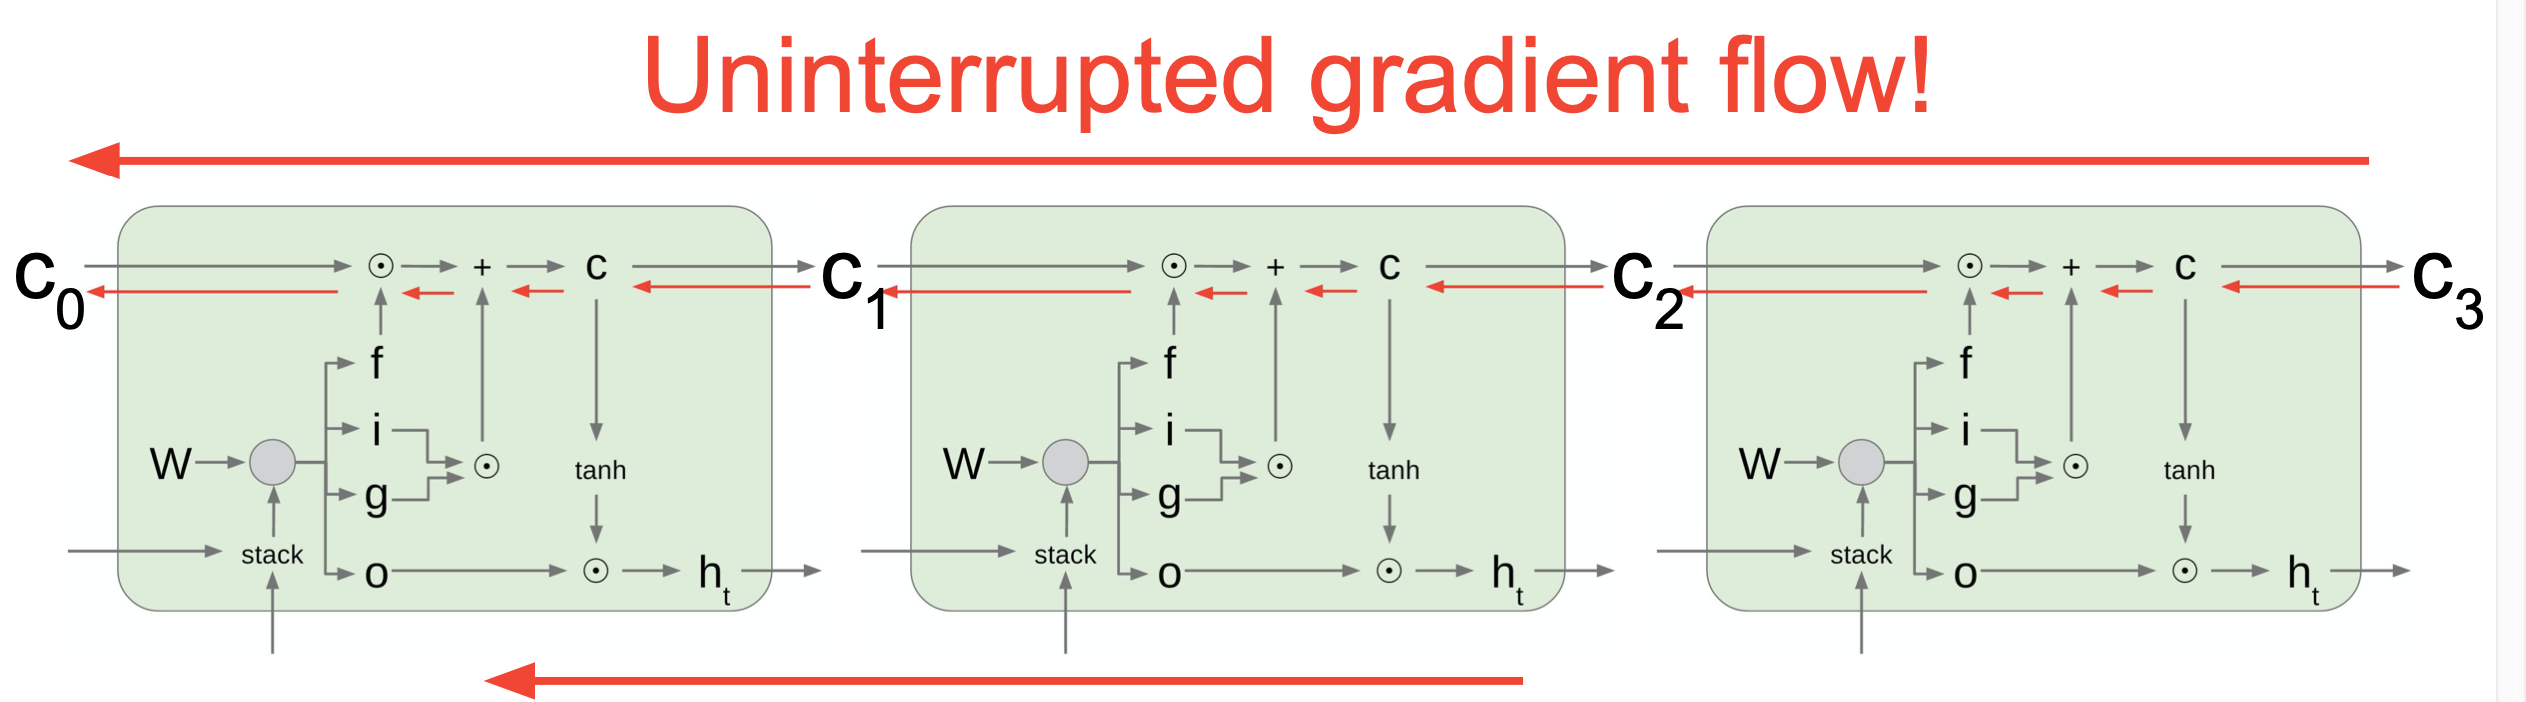
\includegraphics[width=1\textwidth]{fig/flow.png}
       \centering
      \textcolor{Orange}{\textbf{\caption{Figure Description}}}\label{fig:1}
    \end{figure}

\subsubsection{Subsection}

In pretium enim dui, quis ornare odio varius et. Nulla facilisi. Nunc tristique tortor at urna vehicula, elementum bibendum tortor hendrerit. Ut eu risus nisi. Vestibulum nunc lorem, tristique sed ultrices nec, porta et ligula. Nam facilisis felis a congue auctor. Fusce id odio in libero blandit cursus nec nec arcu. Nulla eu ultricies massa, id dapibus nisi. Donec tellus urna, maximus nec semper id, consectetur eu mi. Vestibulum elit eros, porta ac eros a, mattis pulvinar magna. Nulla pellentesque dapibus leo molestie varius. Duis ut rutrum urna, at condimentum dui. Sed orci magna, faucibus nec quam et, malesuada ultrices velit. Nam a lorem a massa facilisis rutrum eget id nunc. Morbi aliquet felis et tincidunt scelerisque. 

% %-------------------------Content------------------------



